\documentclass[1p]{elsarticle_modified}
%\bibliographystyle{elsarticle-num}

%\usepackage[colorlinks]{hyperref}
%\usepackage{abbrmath_seonhwa} %\Abb, \Ascr, \Acal ,\Abf, \Afrak
\usepackage{amsfonts}
\usepackage{amssymb}
\usepackage{amsmath}
\usepackage{amsthm}
\usepackage{scalefnt}
\usepackage{amsbsy}
\usepackage{kotex}
\usepackage{caption}
\usepackage{subfig}
\usepackage{color}
\usepackage{graphicx}
\usepackage{xcolor} %% white, black, red, green, blue, cyan, magenta, yellow
\usepackage{float}
\usepackage{setspace}
\usepackage{hyperref}

\usepackage{tikz}
\usetikzlibrary{arrows}

\usepackage{multirow}
\usepackage{array} % fixed length table
\usepackage{hhline}

%%%%%%%%%%%%%%%%%%%%%
\makeatletter
\renewcommand*\env@matrix[1][\arraystretch]{%
	\edef\arraystretch{#1}%
	\hskip -\arraycolsep
	\let\@ifnextchar\new@ifnextchar
	\array{*\c@MaxMatrixCols c}}
\makeatother %https://tex.stackexchange.com/questions/14071/how-can-i-increase-the-line-spacing-in-a-matrix
%%%%%%%%%%%%%%%

\usepackage[normalem]{ulem}

\newcommand{\msout}[1]{\ifmmode\text{\sout{\ensuremath{#1}}}\else\sout{#1}\fi}
%SOURCE: \msout is \stkout macro in https://tex.stackexchange.com/questions/20609/strikeout-in-math-mode

\newcommand{\cancel}[1]{
	\ifmmode
	{\color{red}\msout{#1}}
	\else
	{\color{red}\sout{#1}}
	\fi
}

\newcommand{\add}[1]{
	{\color{blue}\uwave{#1}}
}

\newcommand{\replace}[2]{
	\ifmmode
	{\color{red}\msout{#1}}{\color{blue}\uwave{#2}}
	\else
	{\color{red}\sout{#1}}{\color{blue}\uwave{#2}}
	\fi
}

\newcommand{\Sol}{\mathcal{S}} %segment
\newcommand{\D}{D} %diagram
\newcommand{\A}{\mathcal{A}} %arc


%%%%%%%%%%%%%%%%%%%%%%%%%%%%%5 test

\def\sl{\operatorname{\textup{SL}}(2,\Cbb)}
\def\psl{\operatorname{\textup{PSL}}(2,\Cbb)}
\def\quan{\mkern 1mu \triangleright \mkern 1mu}

\theoremstyle{definition}
\newtheorem{thm}{Theorem}[section]
\newtheorem{prop}[thm]{Proposition}
\newtheorem{lem}[thm]{Lemma}
\newtheorem{ques}[thm]{Question}
\newtheorem{cor}[thm]{Corollary}
\newtheorem{defn}[thm]{Definition}
\newtheorem{exam}[thm]{Example}
\newtheorem{rmk}[thm]{Remark}
\newtheorem{alg}[thm]{Algorithm}

\newcommand{\I}{\sqrt{-1}}
\begin{document}

%\begin{frontmatter}
%
%\title{Boundary parabolic representations of knots up to 8 crossings}
%
%%% Group authors per affiliation:
%\author{Yunhi Cho} 
%\address{Department of Mathematics, University of Seoul, Seoul, Korea}
%\ead{yhcho@uos.ac.kr}
%
%
%\author{Seonhwa Kim} %\fnref{s_kim}}
%\address{Center for Geometry and Physics, Institute for Basic Science, Pohang, 37673, Korea}
%\ead{ryeona17@ibs.re.kr}
%
%\author{Hyuk Kim}
%\address{Department of Mathematical Sciences, Seoul National University, Seoul 08826, Korea}
%\ead{hyukkim@snu.ac.kr}
%
%\author{Seokbeom Yoon}
%\address{Department of Mathematical Sciences, Seoul National University, Seoul, 08826,  Korea}
%\ead{sbyoon15@snu.ac.kr}
%
%\begin{abstract}
%We find all boundary parabolic representation of knots up to 8 crossings.
%
%\end{abstract}
%\begin{keyword}
%    \MSC[2010] 57M25 
%\end{keyword}
%
%\end{frontmatter}

%\linenumbers
%\tableofcontents
%
\newcommand\colored[1]{\textcolor{white}{\rule[-0.35ex]{0.8em}{1.4ex}}\kern-0.8em\color{red} #1}%
%\newcommand\colored[1]{\textcolor{white}{ #1}\kern-2.17ex	\textcolor{white}{ #1}\kern-1.81ex	\textcolor{white}{ #1}\kern-2.15ex\color{red}#1	}

{\Large $\underline{12a_{0219}~(K12a_{0219})}$}

\setlength{\tabcolsep}{10pt}
\renewcommand{\arraystretch}{1.6}
\vspace{1cm}\begin{tabular}{m{100pt}>{\centering\arraybackslash}m{274pt}}
\multirow{5}{120pt}{
	\centering
	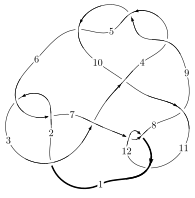
\includegraphics[width=112pt]{../../../GIT/diagram.site/Diagrams/png/1020_12a_0219.png}\\
\ \ \ A knot diagram\footnotemark}&
\allowdisplaybreaks
\textbf{Linearized knot diagam} \\
\cline{2-2}
 &
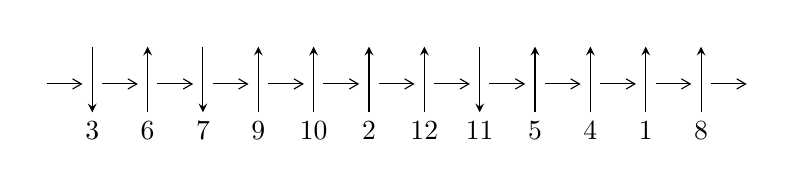
\begin{tikzpicture}[x=20pt, y=17pt]
	% nodes
	\node (C0) at (0, 0) {};
	\node (C1) at (1, 0) {};
	\node (C1U) at (1, +1) {};
	\node (C1D) at (1, -1) {3};

	\node (C2) at (2, 0) {};
	\node (C2U) at (2, +1) {};
	\node (C2D) at (2, -1) {6};

	\node (C3) at (3, 0) {};
	\node (C3U) at (3, +1) {};
	\node (C3D) at (3, -1) {7};

	\node (C4) at (4, 0) {};
	\node (C4U) at (4, +1) {};
	\node (C4D) at (4, -1) {9};

	\node (C5) at (5, 0) {};
	\node (C5U) at (5, +1) {};
	\node (C5D) at (5, -1) {10};

	\node (C6) at (6, 0) {};
	\node (C6U) at (6, +1) {};
	\node (C6D) at (6, -1) {2};

	\node (C7) at (7, 0) {};
	\node (C7U) at (7, +1) {};
	\node (C7D) at (7, -1) {12};

	\node (C8) at (8, 0) {};
	\node (C8U) at (8, +1) {};
	\node (C8D) at (8, -1) {11};

	\node (C9) at (9, 0) {};
	\node (C9U) at (9, +1) {};
	\node (C9D) at (9, -1) {5};

	\node (C10) at (10, 0) {};
	\node (C10U) at (10, +1) {};
	\node (C10D) at (10, -1) {4};

	\node (C11) at (11, 0) {};
	\node (C11U) at (11, +1) {};
	\node (C11D) at (11, -1) {1};

	\node (C12) at (12, 0) {};
	\node (C12U) at (12, +1) {};
	\node (C12D) at (12, -1) {8};
	\node (C13) at (13, 0) {};

	% arrows
	\draw[->,>={angle 60}]
	(C0) edge (C1) (C1) edge (C2) (C2) edge (C3) (C3) edge (C4) (C4) edge (C5) (C5) edge (C6) (C6) edge (C7) (C7) edge (C8) (C8) edge (C9) (C9) edge (C10) (C10) edge (C11) (C11) edge (C12) (C12) edge (C13) ;	\draw[->,>=stealth]
	(C1U) edge (C1D) (C2D) edge (C2U) (C3U) edge (C3D) (C4D) edge (C4U) (C5D) edge (C5U) (C6D) edge (C6U) (C7D) edge (C7U) (C8U) edge (C8D) (C9D) edge (C9U) (C10D) edge (C10U) (C11D) edge (C11U) (C12D) edge (C12U) ;
	\end{tikzpicture} \\
\hhline{~~} \\& 
\textbf{Solving Sequence} \\ \cline{2-2} 
 &
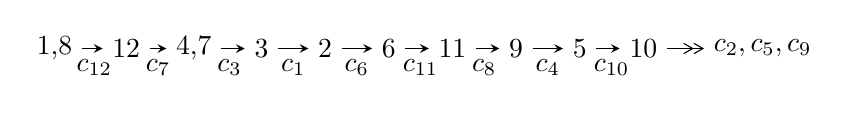
\begin{tikzpicture}[x=23pt, y=7pt]
	% node
	\node (A0) at (-1/8, 0) {1,8};
	\node (A1) at (1, 0) {12};
	\node (A2) at (33/16, 0) {4,7};
	\node (A3) at (25/8, 0) {3};
	\node (A4) at (33/8, 0) {2};
	\node (A5) at (41/8, 0) {6};
	\node (A6) at (49/8, 0) {11};
	\node (A7) at (57/8, 0) {9};
	\node (A8) at (65/8, 0) {5};
	\node (A9) at (73/8, 0) {10};
	\node (C1) at (1/2, -1) {$c_{12}$};
	\node (C2) at (3/2, -1) {$c_{7}$};
	\node (C3) at (21/8, -1) {$c_{3}$};
	\node (C4) at (29/8, -1) {$c_{1}$};
	\node (C5) at (37/8, -1) {$c_{6}$};
	\node (C6) at (45/8, -1) {$c_{11}$};
	\node (C7) at (53/8, -1) {$c_{8}$};
	\node (C8) at (61/8, -1) {$c_{4}$};
	\node (C9) at (69/8, -1) {$c_{10}$};
	\node (A10) at (11, 0) {$c_{2},c_{5},c_{9}$};

	% edge
	\draw[->,>=stealth]	
	(A0) edge (A1) (A1) edge (A2) (A2) edge (A3) (A3) edge (A4) (A4) edge (A5) (A5) edge (A6) (A6) edge (A7) (A7) edge (A8) (A8) edge (A9) ;
	\draw[->>,>={angle 60}]	
	(A9) edge (A10);
\end{tikzpicture} \\ 

\end{tabular} \\

\footnotetext{
The image of knot diagram is generated by the software ``\textbf{Draw programme}" developed by Andrew Bartholomew(\url{http://www.layer8.co.uk/maths/draw/index.htm\#Running-draw}), where we modified some parts for our purpose(\url{https://github.com/CATsTAILs/LinksPainter}).
}\phantom \\ \newline 
\centering \textbf{Ideals for irreducible components\footnotemark of $X_{\text{par}}$} 
 
\begin{align*}
I^u_{1}&=\langle 
-3.29644\times10^{65} u^{95}+8.39309\times10^{65} u^{94}+\cdots+6.47380\times10^{64} b-3.00158\times10^{66},\\
\phantom{I^u_{1}}&\phantom{= \langle  }-3.21501\times10^{65} u^{95}+4.26233\times10^{65} u^{94}+\cdots+2.26583\times10^{65} a+6.65379\times10^{65},\\
\phantom{I^u_{1}}&\phantom{= \langle  }u^{96}-3 u^{95}+\cdots+33 u-7\rangle \\
I^u_{2}&=\langle 
b^2- b+1,\;a^2-2,\;u+1\rangle \\
I^u_{3}&=\langle 
b^2- b+1,\;a,\;u-1\rangle \\
\\
\end{align*}
\raggedright * 3 irreducible components of $\dim_{\mathbb{C}}=0$, with total 102 representations.\\
\footnotetext{All coefficients of polynomials are rational numbers. But the coefficients are sometimes approximated in decimal forms when there is not enough margin.}
\newpage
\renewcommand{\arraystretch}{1}
\centering \section*{I. $I^u_{1}= \langle -3.30\times10^{65} u^{95}+8.39\times10^{65} u^{94}+\cdots+6.47\times10^{64} b-3.00\times10^{66},\;-3.22\times10^{65} u^{95}+4.26\times10^{65} u^{94}+\cdots+2.27\times10^{65} a+6.65\times10^{65},\;u^{96}-3 u^{95}+\cdots+33 u-7 \rangle$}
\flushleft \textbf{(i) Arc colorings}\\
\begin{tabular}{m{7pt} m{180pt} m{7pt} m{180pt} }
\flushright $a_{1}=$&$\begin{pmatrix}1\\0\end{pmatrix}$ \\
\flushright $a_{8}=$&$\begin{pmatrix}0\\u\end{pmatrix}$ \\
\flushright $a_{12}=$&$\begin{pmatrix}1\\u^2\end{pmatrix}$ \\
\flushright $a_{4}=$&$\begin{pmatrix}1.41891 u^{95}-1.88113 u^{94}+\cdots-1.85504 u-2.93658\\5.09198 u^{95}-12.9647 u^{94}+\cdots-163.121 u+46.3650\end{pmatrix}$ \\
\flushright $a_{7}=$&$\begin{pmatrix}- u\\- u^3+u\end{pmatrix}$ \\
\flushright $a_{3}=$&$\begin{pmatrix}2.25748 u^{95}-5.20460 u^{94}+\cdots-43.2293 u+11.0345\\2.44396 u^{95}-6.50914 u^{94}+\cdots-89.2208 u+26.7397\end{pmatrix}$ \\
\flushright $a_{2}=$&$\begin{pmatrix}-1.17179 u^{95}+3.07653 u^{94}+\cdots+25.4465 u-7.56802\\-0.189323 u^{95}+1.36509 u^{94}+\cdots+27.8824 u-10.2921\end{pmatrix}$ \\
\flushright $a_{6}=$&$\begin{pmatrix}-2.25210 u^{95}+5.51531 u^{94}+\cdots+73.2516 u-21.0352\\-1.99587 u^{95}+5.14903 u^{94}+\cdots+88.6507 u-24.4894\end{pmatrix}$ \\
\flushright $a_{11}=$&$\begin{pmatrix}- u^2+1\\u^2\end{pmatrix}$ \\
\flushright $a_{9}=$&$\begin{pmatrix}- u^5+2 u^3- u\\u^5- u^3+u\end{pmatrix}$ \\
\flushright $a_{5}=$&$\begin{pmatrix}1.21133 u^{95}-0.874118 u^{94}+\cdots+25.5221 u-12.9364\\3.51190 u^{95}-9.39402 u^{94}+\cdots-126.246 u+37.7277\end{pmatrix}$ \\
\flushright $a_{10}=$&$\begin{pmatrix}-0.362137 u^{95}+0.883926 u^{94}+\cdots-4.63087 u+1.81548\\-1.74806 u^{95}+3.53499 u^{94}+\cdots+51.1345 u-14.0192\end{pmatrix}$\\&\end{tabular}
\flushleft \textbf{(ii) Obstruction class $= -1$}\\~\\
\flushleft \textbf{(iii) Cusp Shapes $= -3.60410 u^{95}+10.8203 u^{94}+\cdots+117.107 u-19.1541$}\\~\\
\newpage\renewcommand{\arraystretch}{1}
\flushleft \textbf{(iv) u-Polynomials at the component}\newline \\
\begin{tabular}{m{50pt}|m{274pt}}
Crossings & \hspace{64pt}u-Polynomials at each crossing \\
\hline $$\begin{aligned}c_{1}\end{aligned}$$&$\begin{aligned}
&u^{96}+44 u^{95}+\cdots-24 u+1
\end{aligned}$\\
\hline $$\begin{aligned}c_{2},c_{6}\end{aligned}$$&$\begin{aligned}
&u^{96}-2 u^{95}+\cdots-10 u+1
\end{aligned}$\\
\hline $$\begin{aligned}c_{3}\end{aligned}$$&$\begin{aligned}
&u^{96}+2 u^{95}+\cdots+170 u+29
\end{aligned}$\\
\hline $$\begin{aligned}c_{4},c_{5},c_{9}\end{aligned}$$&$\begin{aligned}
&u^{96}+u^{95}+\cdots+12 u-4
\end{aligned}$\\
\hline $$\begin{aligned}c_{7},c_{12}\end{aligned}$$&$\begin{aligned}
&u^{96}-3 u^{95}+\cdots+33 u-7
\end{aligned}$\\
\hline $$\begin{aligned}c_{8}\end{aligned}$$&$\begin{aligned}
&u^{96}-15 u^{95}+\cdots-17408 u+1792
\end{aligned}$\\
\hline $$\begin{aligned}c_{10}\end{aligned}$$&$\begin{aligned}
&u^{96}-3 u^{95}+\cdots+4692 u+9292
\end{aligned}$\\
\hline $$\begin{aligned}c_{11}\end{aligned}$$&$\begin{aligned}
&u^{96}-53 u^{95}+\cdots-417 u+49
\end{aligned}$\\
\hline
\end{tabular}\\~\\
\newpage\renewcommand{\arraystretch}{1}
\flushleft \textbf{(v) Riley Polynomials at the component}\newline \\
\begin{tabular}{m{50pt}|m{274pt}}
Crossings & \hspace{64pt}Riley Polynomials at each crossing \\
\hline $$\begin{aligned}c_{1}\end{aligned}$$&$\begin{aligned}
&y^{96}+20 y^{95}+\cdots-640 y+1
\end{aligned}$\\
\hline $$\begin{aligned}c_{2},c_{6}\end{aligned}$$&$\begin{aligned}
&y^{96}+44 y^{95}+\cdots-24 y+1
\end{aligned}$\\
\hline $$\begin{aligned}c_{3}\end{aligned}$$&$\begin{aligned}
&y^{96}-4 y^{95}+\cdots-69036 y+841
\end{aligned}$\\
\hline $$\begin{aligned}c_{4},c_{5},c_{9}\end{aligned}$$&$\begin{aligned}
&y^{96}-91 y^{95}+\cdots+240 y+16
\end{aligned}$\\
\hline $$\begin{aligned}c_{7},c_{12}\end{aligned}$$&$\begin{aligned}
&y^{96}-53 y^{95}+\cdots-417 y+49
\end{aligned}$\\
\hline $$\begin{aligned}c_{8}\end{aligned}$$&$\begin{aligned}
&y^{96}+61 y^{95}+\cdots-128483328 y+3211264
\end{aligned}$\\
\hline $$\begin{aligned}c_{10}\end{aligned}$$&$\begin{aligned}
&y^{96}-31 y^{95}+\cdots-573141968 y+86341264
\end{aligned}$\\
\hline $$\begin{aligned}c_{11}\end{aligned}$$&$\begin{aligned}
&y^{96}-13 y^{95}+\cdots-80985 y+2401
\end{aligned}$\\
\hline
\end{tabular}\\~\\
\newpage\flushleft \textbf{(vi) Complex Volumes and Cusp Shapes}
$$\begin{array}{c|c|c}  
\text{Solutions to }I^u_{1}& \I (\text{vol} + \sqrt{-1}CS) & \text{Cusp shape}\\
 \hline 
\begin{aligned}
u &= \phantom{-}0.833148 + 0.623345 I \\
a &= -0.031613 + 0.759344 I \\
b &= -0.078546 - 0.988047 I\end{aligned}
 & -1.40395 + 2.16811 I & \phantom{-0.000000 } 0 \\ \hline\begin{aligned}
u &= \phantom{-}0.833148 - 0.623345 I \\
a &= -0.031613 - 0.759344 I \\
b &= -0.078546 + 0.988047 I\end{aligned}
 & -1.40395 - 2.16811 I & \phantom{-0.000000 } 0 \\ \hline\begin{aligned}
u &= -1.013030 + 0.253365 I \\
a &= -1.17454 - 1.24265 I \\
b &= -0.353670 + 0.324350 I\end{aligned}
 & \phantom{-}6.33381 + 0.37203 I & \phantom{-0.000000 } 0 \\ \hline\begin{aligned}
u &= -1.013030 - 0.253365 I \\
a &= -1.17454 + 1.24265 I \\
b &= -0.353670 - 0.324350 I\end{aligned}
 & \phantom{-}6.33381 - 0.37203 I & \phantom{-0.000000 } 0 \\ \hline\begin{aligned}
u &= -0.847878 + 0.624079 I \\
a &= \phantom{-}0.820203 + 0.073555 I \\
b &= \phantom{-}0.173341 + 0.046759 I\end{aligned}
 & -4.59002 - 6.24024 I & \phantom{-0.000000 } 0 \\ \hline\begin{aligned}
u &= -0.847878 - 0.624079 I \\
a &= \phantom{-}0.820203 - 0.073555 I \\
b &= \phantom{-}0.173341 - 0.046759 I\end{aligned}
 & -4.59002 + 6.24024 I & \phantom{-0.000000 } 0 \\ \hline\begin{aligned}
u &= -0.689352 + 0.647691 I \\
a &= \phantom{-}0.429393 - 0.447615 I \\
b &= \phantom{-}0.126999 + 0.557750 I\end{aligned}
 & -5.04287 + 1.33222 I & \phantom{-0.000000 } 0 \\ \hline\begin{aligned}
u &= -0.689352 - 0.647691 I \\
a &= \phantom{-}0.429393 + 0.447615 I \\
b &= \phantom{-}0.126999 - 0.557750 I\end{aligned}
 & -5.04287 - 1.33222 I & \phantom{-0.000000 } 0 \\ \hline\begin{aligned}
u &= -0.778350 + 0.535879 I \\
a &= -0.416102 - 0.047250 I \\
b &= -0.407471 - 0.336585 I\end{aligned}
 & -1.74499 - 2.16540 I & \phantom{-0.000000 } 0 \\ \hline\begin{aligned}
u &= -0.778350 - 0.535879 I \\
a &= -0.416102 + 0.047250 I \\
b &= -0.407471 + 0.336585 I\end{aligned}
 & -1.74499 + 2.16540 I & \phantom{-0.000000 } 0\\
 \hline 
 \end{array}$$\newpage$$\begin{array}{c|c|c}  
\text{Solutions to }I^u_{1}& \I (\text{vol} + \sqrt{-1}CS) & \text{Cusp shape}\\
 \hline 
\begin{aligned}
u &= \phantom{-}0.916273 + 0.567375 I \\
a &= -0.091728 - 0.259844 I \\
b &= -0.228304 + 0.883380 I\end{aligned}
 & \phantom{-}2.43863 + 5.37302 I & \phantom{-0.000000 } 0 \\ \hline\begin{aligned}
u &= \phantom{-}0.916273 - 0.567375 I \\
a &= -0.091728 + 0.259844 I \\
b &= -0.228304 - 0.883380 I\end{aligned}
 & \phantom{-}2.43863 - 5.37302 I & \phantom{-0.000000 } 0 \\ \hline\begin{aligned}
u &= \phantom{-}0.677177 + 0.623662 I \\
a &= \phantom{-}1.081130 - 0.584442 I \\
b &= \phantom{-}0.047616 + 0.542990 I\end{aligned}
 & -1.82843 + 2.68030 I & \phantom{-0.000000 } 0 \\ \hline\begin{aligned}
u &= \phantom{-}0.677177 - 0.623662 I \\
a &= \phantom{-}1.081130 + 0.584442 I \\
b &= \phantom{-}0.047616 - 0.542990 I\end{aligned}
 & -1.82843 - 2.68030 I & \phantom{-0.000000 } 0 \\ \hline\begin{aligned}
u &= \phantom{-}0.829088 + 0.385457 I \\
a &= \phantom{-}0.683999 - 0.152464 I \\
b &= \phantom{-}0.17609 + 1.90497 I\end{aligned}
 & \phantom{-}5.09287 + 4.15151 I & \phantom{-}10.22388 - 7.48444 I \\ \hline\begin{aligned}
u &= \phantom{-}0.829088 - 0.385457 I \\
a &= \phantom{-}0.683999 + 0.152464 I \\
b &= \phantom{-}0.17609 - 1.90497 I\end{aligned}
 & \phantom{-}5.09287 - 4.15151 I & \phantom{-}10.22388 + 7.48444 I \\ \hline\begin{aligned}
u &= \phantom{-}0.169868 + 0.894100 I \\
a &= \phantom{-}1.78018 - 1.18389 I \\
b &= -1.50343 + 1.33301 I\end{aligned}
 & \phantom{-}4.56609 - 11.26670 I & \phantom{-}6.00000 + 7.26947 I \\ \hline\begin{aligned}
u &= \phantom{-}0.169868 - 0.894100 I \\
a &= \phantom{-}1.78018 + 1.18389 I \\
b &= -1.50343 - 1.33301 I\end{aligned}
 & \phantom{-}4.56609 + 11.26670 I & \phantom{-}6.00000 - 7.26947 I \\ \hline\begin{aligned}
u &= -1.09363\phantom{ +0.000000I} \\
a &= -1.01722\phantom{ +0.000000I} \\
b &= -0.00371003\phantom{ +0.000000I}\end{aligned}
 & \phantom{-}6.50487\phantom{ +0.000000I} & \phantom{-0.000000 } 0 \\ \hline\begin{aligned}
u &= \phantom{-}0.544581 + 0.708967 I \\
a &= \phantom{-}0.845405 - 0.041621 I \\
b &= \phantom{-}0.142315 - 0.016053 I\end{aligned}
 & -1.40901 - 4.80978 I & \phantom{-}3.29593 + 4.34029 I\\
 \hline 
 \end{array}$$\newpage$$\begin{array}{c|c|c}  
\text{Solutions to }I^u_{1}& \I (\text{vol} + \sqrt{-1}CS) & \text{Cusp shape}\\
 \hline 
\begin{aligned}
u &= \phantom{-}0.544581 - 0.708967 I \\
a &= \phantom{-}0.845405 + 0.041621 I \\
b &= \phantom{-}0.142315 + 0.016053 I\end{aligned}
 & -1.40901 + 4.80978 I & \phantom{-}3.29593 - 4.34029 I \\ \hline\begin{aligned}
u &= \phantom{-}1.025840 + 0.457928 I \\
a &= -0.401083 + 1.281920 I \\
b &= -0.818475 - 0.717111 I\end{aligned}
 & -0.179654 + 1.344070 I & \phantom{-0.000000 } 0 \\ \hline\begin{aligned}
u &= \phantom{-}1.025840 - 0.457928 I \\
a &= -0.401083 - 1.281920 I \\
b &= -0.818475 + 0.717111 I\end{aligned}
 & -0.179654 - 1.344070 I & \phantom{-0.000000 } 0 \\ \hline\begin{aligned}
u &= \phantom{-}0.151562 + 0.857368 I \\
a &= -1.84928 + 0.82401 I \\
b &= \phantom{-}1.56139 - 1.12610 I\end{aligned}
 & \phantom{-}6.64562 - 6.08638 I & \phantom{-}10.39988 + 3.13837 I \\ \hline\begin{aligned}
u &= \phantom{-}0.151562 - 0.857368 I \\
a &= -1.84928 - 0.82401 I \\
b &= \phantom{-}1.56139 + 1.12610 I\end{aligned}
 & \phantom{-}6.64562 + 6.08638 I & \phantom{-}10.39988 - 3.13837 I \\ \hline\begin{aligned}
u &= \phantom{-}0.952434 + 0.625237 I \\
a &= \phantom{-}0.483461 + 0.314958 I \\
b &= \phantom{-}0.068470 - 0.575431 I\end{aligned}
 & -0.24974 + 9.86654 I & \phantom{-0.000000 } 0 \\ \hline\begin{aligned}
u &= \phantom{-}0.952434 - 0.625237 I \\
a &= \phantom{-}0.483461 - 0.314958 I \\
b &= \phantom{-}0.068470 + 0.575431 I\end{aligned}
 & -0.24974 - 9.86654 I & \phantom{-0.000000 } 0 \\ \hline\begin{aligned}
u &= -0.208680 + 0.830969 I \\
a &= \phantom{-}1.72886 + 0.97902 I \\
b &= -1.16298 - 0.97853 I\end{aligned}
 & -1.15634 + 7.77416 I & \phantom{-}3.13699 - 7.30330 I \\ \hline\begin{aligned}
u &= -0.208680 - 0.830969 I \\
a &= \phantom{-}1.72886 - 0.97902 I \\
b &= -1.16298 + 0.97853 I\end{aligned}
 & -1.15634 - 7.77416 I & \phantom{-}3.13699 + 7.30330 I \\ \hline\begin{aligned}
u &= \phantom{-}1.141790 + 0.090770 I \\
a &= \phantom{-}0.066259 + 0.276876 I \\
b &= -0.385873 + 0.580683 I\end{aligned}
 & \phantom{-}1.11225 + 1.53245 I & \phantom{-0.000000 } 0\\
 \hline 
 \end{array}$$\newpage$$\begin{array}{c|c|c}  
\text{Solutions to }I^u_{1}& \I (\text{vol} + \sqrt{-1}CS) & \text{Cusp shape}\\
 \hline 
\begin{aligned}
u &= \phantom{-}1.141790 - 0.090770 I \\
a &= \phantom{-}0.066259 - 0.276876 I \\
b &= -0.385873 - 0.580683 I\end{aligned}
 & \phantom{-}1.11225 - 1.53245 I & \phantom{-0.000000 } 0 \\ \hline\begin{aligned}
u &= \phantom{-}0.235538 + 0.804768 I \\
a &= \phantom{-}1.066780 - 0.567870 I \\
b &= -1.14823 + 0.91773 I\end{aligned}
 & \phantom{-}1.68291 - 3.82528 I & \phantom{-}4.02618 + 2.15723 I \\ \hline\begin{aligned}
u &= \phantom{-}0.235538 - 0.804768 I \\
a &= \phantom{-}1.066780 + 0.567870 I \\
b &= -1.14823 - 0.91773 I\end{aligned}
 & \phantom{-}1.68291 + 3.82528 I & \phantom{-}4.02618 - 2.15723 I \\ \hline\begin{aligned}
u &= \phantom{-}0.743530 + 0.335556 I \\
a &= -0.888754 + 0.289225 I \\
b &= -0.90209 - 1.75209 I\end{aligned}
 & \phantom{-}4.78693 - 0.88146 I & \phantom{-}8.78250 - 0.86023 I \\ \hline\begin{aligned}
u &= \phantom{-}0.743530 - 0.335556 I \\
a &= -0.888754 - 0.289225 I \\
b &= -0.90209 + 1.75209 I\end{aligned}
 & \phantom{-}4.78693 + 0.88146 I & \phantom{-}8.78250 + 0.86023 I \\ \hline\begin{aligned}
u &= \phantom{-}0.553648 + 0.598382 I \\
a &= -0.746834 + 0.434809 I \\
b &= -0.417163 - 0.310845 I\end{aligned}
 & \phantom{-}1.43855 - 0.78309 I & \phantom{-}7.25184 + 0.14491 I \\ \hline\begin{aligned}
u &= \phantom{-}0.553648 - 0.598382 I \\
a &= -0.746834 - 0.434809 I \\
b &= -0.417163 + 0.310845 I\end{aligned}
 & \phantom{-}1.43855 + 0.78309 I & \phantom{-}7.25184 - 0.14491 I \\ \hline\begin{aligned}
u &= -1.136260 + 0.381382 I \\
a &= \phantom{-}0.142180 - 1.031870 I \\
b &= -2.00804 + 0.36080 I\end{aligned}
 & \phantom{-}3.39912 + 0.40632 I & \phantom{-0.000000 } 0 \\ \hline\begin{aligned}
u &= -1.136260 - 0.381382 I \\
a &= \phantom{-}0.142180 + 1.031870 I \\
b &= -2.00804 - 0.36080 I\end{aligned}
 & \phantom{-}3.39912 - 0.40632 I & \phantom{-0.000000 } 0 \\ \hline\begin{aligned}
u &= -0.169433 + 0.771054 I \\
a &= -1.68605 - 0.64191 I \\
b &= \phantom{-}1.102480 + 0.759939 I\end{aligned}
 & \phantom{-}0.90397 + 2.82486 I & \phantom{-}6.31873 - 3.40690 I\\
 \hline 
 \end{array}$$\newpage$$\begin{array}{c|c|c}  
\text{Solutions to }I^u_{1}& \I (\text{vol} + \sqrt{-1}CS) & \text{Cusp shape}\\
 \hline 
\begin{aligned}
u &= -0.169433 - 0.771054 I \\
a &= -1.68605 + 0.64191 I \\
b &= \phantom{-}1.102480 - 0.759939 I\end{aligned}
 & \phantom{-}0.90397 - 2.82486 I & \phantom{-}6.31873 + 3.40690 I \\ \hline\begin{aligned}
u &= -1.183880 + 0.262794 I \\
a &= -0.211510 - 0.942755 I \\
b &= -0.773464 - 0.301090 I\end{aligned}
 & \phantom{-}6.17767 + 0.42669 I & \phantom{-0.000000 } 0 \\ \hline\begin{aligned}
u &= -1.183880 - 0.262794 I \\
a &= -0.211510 + 0.942755 I \\
b &= -0.773464 + 0.301090 I\end{aligned}
 & \phantom{-}6.17767 - 0.42669 I & \phantom{-0.000000 } 0 \\ \hline\begin{aligned}
u &= -0.332091 + 0.705976 I \\
a &= \phantom{-}0.954112 + 0.762646 I \\
b &= -0.681852 - 0.899696 I\end{aligned}
 & -3.49407 + 0.59180 I & -1.16788 - 1.13897 I \\ \hline\begin{aligned}
u &= -0.332091 - 0.705976 I \\
a &= \phantom{-}0.954112 - 0.762646 I \\
b &= -0.681852 + 0.899696 I\end{aligned}
 & -3.49407 - 0.59180 I & -1.16788 + 1.13897 I \\ \hline\begin{aligned}
u &= -1.107690 + 0.529396 I \\
a &= -0.498342 - 1.265020 I \\
b &= -1.25300 + 0.94720 I\end{aligned}
 & -1.22305 - 5.30620 I & \phantom{-0.000000 } 0 \\ \hline\begin{aligned}
u &= -1.107690 - 0.529396 I \\
a &= -0.498342 + 1.265020 I \\
b &= -1.25300 - 0.94720 I\end{aligned}
 & -1.22305 + 5.30620 I & \phantom{-0.000000 } 0 \\ \hline\begin{aligned}
u &= -1.152600 + 0.431449 I \\
a &= -0.027714 + 1.227330 I \\
b &= \phantom{-}1.91070 - 0.67274 I\end{aligned}
 & \phantom{-}4.71563 - 4.76508 I & \phantom{-0.000000 } 0 \\ \hline\begin{aligned}
u &= -1.152600 - 0.431449 I \\
a &= -0.027714 - 1.227330 I \\
b &= \phantom{-}1.91070 + 0.67274 I\end{aligned}
 & \phantom{-}4.71563 + 4.76508 I & \phantom{-0.000000 } 0 \\ \hline\begin{aligned}
u &= -0.758438 + 0.093448 I \\
a &= \phantom{-}0.022205 - 0.320943 I \\
b &= -0.39857 - 1.36361 I\end{aligned}
 & \phantom{-}1.01410 - 2.32335 I & \phantom{-}0.25395 + 5.97647 I\\
 \hline 
 \end{array}$$\newpage$$\begin{array}{c|c|c}  
\text{Solutions to }I^u_{1}& \I (\text{vol} + \sqrt{-1}CS) & \text{Cusp shape}\\
 \hline 
\begin{aligned}
u &= -0.758438 - 0.093448 I \\
a &= \phantom{-}0.022205 + 0.320943 I \\
b &= -0.39857 + 1.36361 I\end{aligned}
 & \phantom{-}1.01410 + 2.32335 I & \phantom{-}0.25395 - 5.97647 I \\ \hline\begin{aligned}
u &= \phantom{-}0.532506 + 0.546720 I \\
a &= \phantom{-}1.18685 - 0.89970 I \\
b &= -0.268310 + 0.658554 I\end{aligned}
 & -1.65174 + 2.71583 I & \phantom{-}3.09718 - 5.37796 I \\ \hline\begin{aligned}
u &= \phantom{-}0.532506 - 0.546720 I \\
a &= \phantom{-}1.18685 + 0.89970 I \\
b &= -0.268310 - 0.658554 I\end{aligned}
 & -1.65174 - 2.71583 I & \phantom{-}3.09718 + 5.37796 I \\ \hline\begin{aligned}
u &= \phantom{-}1.149740 + 0.466998 I \\
a &= -0.08653 - 1.56454 I \\
b &= \phantom{-}1.41799 + 0.75095 I\end{aligned}
 & \phantom{-}4.46471 + 3.33536 I & \phantom{-0.000000 } 0 \\ \hline\begin{aligned}
u &= \phantom{-}1.149740 - 0.466998 I \\
a &= -0.08653 + 1.56454 I \\
b &= \phantom{-}1.41799 - 0.75095 I\end{aligned}
 & \phantom{-}4.46471 - 3.33536 I & \phantom{-0.000000 } 0 \\ \hline\begin{aligned}
u &= -1.160400 + 0.445571 I \\
a &= \phantom{-}0.19152 - 2.26758 I \\
b &= -1.68333 + 0.56518 I\end{aligned}
 & \phantom{-}9.35943 - 5.74731 I & \phantom{-0.000000 } 0 \\ \hline\begin{aligned}
u &= -1.160400 - 0.445571 I \\
a &= \phantom{-}0.19152 + 2.26758 I \\
b &= -1.68333 - 0.56518 I\end{aligned}
 & \phantom{-}9.35943 + 5.74731 I & \phantom{-0.000000 } 0 \\ \hline\begin{aligned}
u &= \phantom{-}1.189600 + 0.361483 I \\
a &= -0.379797 - 1.089120 I \\
b &= \phantom{-}1.48015 + 0.10596 I\end{aligned}
 & \phantom{-}4.92234 + 0.91841 I & \phantom{-0.000000 } 0 \\ \hline\begin{aligned}
u &= \phantom{-}1.189600 - 0.361483 I \\
a &= -0.379797 + 1.089120 I \\
b &= \phantom{-}1.48015 - 0.10596 I\end{aligned}
 & \phantom{-}4.92234 - 0.91841 I & \phantom{-0.000000 } 0 \\ \hline\begin{aligned}
u &= \phantom{-}1.162430 + 0.455623 I \\
a &= \phantom{-}0.141375 + 1.343700 I \\
b &= -2.62084 - 0.26113 I\end{aligned}
 & \phantom{-}9.28641 + 2.49542 I & \phantom{-0.000000 } 0\\
 \hline 
 \end{array}$$\newpage$$\begin{array}{c|c|c}  
\text{Solutions to }I^u_{1}& \I (\text{vol} + \sqrt{-1}CS) & \text{Cusp shape}\\
 \hline 
\begin{aligned}
u &= \phantom{-}1.162430 - 0.455623 I \\
a &= \phantom{-}0.141375 - 1.343700 I \\
b &= -2.62084 + 0.26113 I\end{aligned}
 & \phantom{-}9.28641 - 2.49542 I & \phantom{-0.000000 } 0 \\ \hline\begin{aligned}
u &= -1.248650 + 0.054886 I \\
a &= \phantom{-}0.566268 + 0.055471 I \\
b &= -0.378813 + 0.353408 I\end{aligned}
 & \phantom{-}4.46285 + 3.16912 I & \phantom{-0.000000 } 0 \\ \hline\begin{aligned}
u &= -1.248650 - 0.054886 I \\
a &= \phantom{-}0.566268 - 0.055471 I \\
b &= -0.378813 - 0.353408 I\end{aligned}
 & \phantom{-}4.46285 - 3.16912 I & \phantom{-0.000000 } 0 \\ \hline\begin{aligned}
u &= \phantom{-}0.076061 + 0.746002 I \\
a &= -2.12820 - 0.24592 I \\
b &= \phantom{-}1.72448 - 0.58053 I\end{aligned}
 & \phantom{-}7.47114 - 3.38666 I & \phantom{-}11.17915 + 3.06622 I \\ \hline\begin{aligned}
u &= \phantom{-}0.076061 - 0.746002 I \\
a &= -2.12820 + 0.24592 I \\
b &= \phantom{-}1.72448 + 0.58053 I\end{aligned}
 & \phantom{-}7.47114 + 3.38666 I & \phantom{-}11.17915 - 3.06622 I \\ \hline\begin{aligned}
u &= -0.710618 + 0.222937 I \\
a &= \phantom{-}2.84990 + 1.22868 I \\
b &= -0.486988 - 0.496637 I\end{aligned}
 & \phantom{-}5.29177 - 2.78792 I & \phantom{-}5.68134 + 6.43519 I \\ \hline\begin{aligned}
u &= -0.710618 - 0.222937 I \\
a &= \phantom{-}2.84990 - 1.22868 I \\
b &= -0.486988 + 0.496637 I\end{aligned}
 & \phantom{-}5.29177 + 2.78792 I & \phantom{-}5.68134 - 6.43519 I \\ \hline\begin{aligned}
u &= \phantom{-}1.147800 + 0.509147 I \\
a &= -0.01264 + 1.77308 I \\
b &= -1.41262 - 1.00296 I\end{aligned}
 & \phantom{-}2.47708 + 8.39381 I & \phantom{-0.000000 } 0 \\ \hline\begin{aligned}
u &= \phantom{-}1.147800 - 0.509147 I \\
a &= -0.01264 - 1.77308 I \\
b &= -1.41262 + 1.00296 I\end{aligned}
 & \phantom{-}2.47708 - 8.39381 I & \phantom{-0.000000 } 0 \\ \hline\begin{aligned}
u &= -1.186860 + 0.415943 I \\
a &= -0.31953 + 1.94554 I \\
b &= \phantom{-}1.67441 - 0.24564 I\end{aligned}
 & \phantom{-}11.10360 - 0.67190 I & \phantom{-0.000000 } 0\\
 \hline 
 \end{array}$$\newpage$$\begin{array}{c|c|c}  
\text{Solutions to }I^u_{1}& \I (\text{vol} + \sqrt{-1}CS) & \text{Cusp shape}\\
 \hline 
\begin{aligned}
u &= -1.186860 - 0.415943 I \\
a &= -0.31953 - 1.94554 I \\
b &= \phantom{-}1.67441 + 0.24564 I\end{aligned}
 & \phantom{-}11.10360 + 0.67190 I & \phantom{-0.000000 } 0 \\ \hline\begin{aligned}
u &= \phantom{-}1.224250 + 0.315936 I \\
a &= \phantom{-}0.527394 + 0.867241 I \\
b &= -1.52114 + 0.23127 I\end{aligned}
 & \phantom{-}3.32134 - 4.02982 I & \phantom{-0.000000 } 0 \\ \hline\begin{aligned}
u &= \phantom{-}1.224250 - 0.315936 I \\
a &= \phantom{-}0.527394 - 0.867241 I \\
b &= -1.52114 - 0.23127 I\end{aligned}
 & \phantom{-}3.32134 + 4.02982 I & \phantom{-0.000000 } 0 \\ \hline\begin{aligned}
u &= \phantom{-}1.181230 + 0.479601 I \\
a &= \phantom{-}0.03534 - 1.49444 I \\
b &= \phantom{-}2.48059 + 0.68389 I\end{aligned}
 & \phantom{-}10.65330 + 7.89324 I & \phantom{-0.000000 } 0 \\ \hline\begin{aligned}
u &= \phantom{-}1.181230 - 0.479601 I \\
a &= \phantom{-}0.03534 + 1.49444 I \\
b &= \phantom{-}2.48059 - 0.68389 I\end{aligned}
 & \phantom{-}10.65330 - 7.89324 I & \phantom{-0.000000 } 0 \\ \hline\begin{aligned}
u &= \phantom{-}0.205507 + 0.689673 I \\
a &= \phantom{-}1.94053 - 0.63363 I \\
b &= -1.040730 + 0.293972 I\end{aligned}
 & -0.23085 - 3.80697 I & \phantom{-}4.88666 + 1.57735 I \\ \hline\begin{aligned}
u &= \phantom{-}0.205507 - 0.689673 I \\
a &= \phantom{-}1.94053 + 0.63363 I \\
b &= -1.040730 - 0.293972 I\end{aligned}
 & -0.23085 + 3.80697 I & \phantom{-}4.88666 - 1.57735 I \\ \hline\begin{aligned}
u &= -1.174460 + 0.516668 I \\
a &= \phantom{-}0.27953 + 1.57255 I \\
b &= \phantom{-}1.64809 - 1.22675 I\end{aligned}
 & \phantom{-}3.83716 - 7.60793 I & \phantom{-0.000000 } 0 \\ \hline\begin{aligned}
u &= -1.174460 - 0.516668 I \\
a &= \phantom{-}0.27953 - 1.57255 I \\
b &= \phantom{-}1.64809 + 1.22675 I\end{aligned}
 & \phantom{-}3.83716 + 7.60793 I & \phantom{-0.000000 } 0 \\ \hline\begin{aligned}
u &= \phantom{-}1.166830 + 0.541752 I \\
a &= -0.53799 + 1.34809 I \\
b &= -1.62687 - 0.92797 I\end{aligned}
 & \phantom{-}4.44082 + 8.81310 I & \phantom{-0.000000 } 0\\
 \hline 
 \end{array}$$\newpage$$\begin{array}{c|c|c}  
\text{Solutions to }I^u_{1}& \I (\text{vol} + \sqrt{-1}CS) & \text{Cusp shape}\\
 \hline 
\begin{aligned}
u &= \phantom{-}1.166830 - 0.541752 I \\
a &= -0.53799 - 1.34809 I \\
b &= -1.62687 + 0.92797 I\end{aligned}
 & \phantom{-}4.44082 - 8.81310 I & \phantom{-0.000000 } 0 \\ \hline\begin{aligned}
u &= -1.184600 + 0.543438 I \\
a &= -0.39453 - 1.70602 I \\
b &= -1.56068 + 1.42955 I\end{aligned}
 & \phantom{-}1.74398 - 12.83170 I & \phantom{-0.000000 } 0 \\ \hline\begin{aligned}
u &= -1.184600 - 0.543438 I \\
a &= -0.39453 + 1.70602 I \\
b &= -1.56068 - 1.42955 I\end{aligned}
 & \phantom{-}1.74398 + 12.83170 I & \phantom{-0.000000 } 0 \\ \hline\begin{aligned}
u &= -1.253330 + 0.364907 I \\
a &= -0.61750 + 1.29425 I \\
b &= \phantom{-}1.65687 + 0.45442 I\end{aligned}
 & \phantom{-}10.99980 + 1.93342 I & \phantom{-0.000000 } 0 \\ \hline\begin{aligned}
u &= -1.253330 - 0.364907 I \\
a &= -0.61750 - 1.29425 I \\
b &= \phantom{-}1.65687 - 0.45442 I\end{aligned}
 & \phantom{-}10.99980 - 1.93342 I & \phantom{-0.000000 } 0 \\ \hline\begin{aligned}
u &= \phantom{-}1.209640 + 0.530526 I \\
a &= \phantom{-}0.47272 - 1.73333 I \\
b &= \phantom{-}2.02520 + 1.40057 I\end{aligned}
 & \phantom{-}9.8052 + 11.1431 I & \phantom{-0.000000 } 0 \\ \hline\begin{aligned}
u &= \phantom{-}1.209640 - 0.530526 I \\
a &= \phantom{-}0.47272 + 1.73333 I \\
b &= \phantom{-}2.02520 - 1.40057 I\end{aligned}
 & \phantom{-}9.8052 - 11.1431 I & \phantom{-0.000000 } 0 \\ \hline\begin{aligned}
u &= -1.283030 + 0.349613 I \\
a &= \phantom{-}0.745627 - 1.039810 I \\
b &= -1.65372 - 0.75490 I\end{aligned}
 & \phantom{-}9.16807 + 7.02990 I & \phantom{-0.000000 } 0 \\ \hline\begin{aligned}
u &= -1.283030 - 0.349613 I \\
a &= \phantom{-}0.745627 + 1.039810 I \\
b &= -1.65372 + 0.75490 I\end{aligned}
 & \phantom{-}9.16807 - 7.02990 I & \phantom{-0.000000 } 0 \\ \hline\begin{aligned}
u &= \phantom{-}0.020929 + 0.667902 I \\
a &= \phantom{-}2.28885 + 0.95053 I \\
b &= -1.75702 + 0.28266 I\end{aligned}
 & \phantom{-}6.12891 + 1.67907 I & \phantom{-}8.89545 - 2.29940 I\\
 \hline 
 \end{array}$$\newpage$$\begin{array}{c|c|c}  
\text{Solutions to }I^u_{1}& \I (\text{vol} + \sqrt{-1}CS) & \text{Cusp shape}\\
 \hline 
\begin{aligned}
u &= \phantom{-}0.020929 - 0.667902 I \\
a &= \phantom{-}2.28885 - 0.95053 I \\
b &= -1.75702 - 0.28266 I\end{aligned}
 & \phantom{-}6.12891 - 1.67907 I & \phantom{-}8.89545 + 2.29940 I \\ \hline\begin{aligned}
u &= \phantom{-}1.219260 + 0.547288 I \\
a &= -0.63482 + 1.81504 I \\
b &= -1.85826 - 1.62972 I\end{aligned}
 & \phantom{-}7.7267 + 16.4978 I & \phantom{-0.000000 } 0 \\ \hline\begin{aligned}
u &= \phantom{-}1.219260 - 0.547288 I \\
a &= -0.63482 - 1.81504 I \\
b &= -1.85826 + 1.62972 I\end{aligned}
 & \phantom{-}7.7267 - 16.4978 I & \phantom{-0.000000 } 0 \\ \hline\begin{aligned}
u &= \phantom{-}0.048425 + 0.646342 I \\
a &= -1.78755 + 0.22856 I \\
b &= \phantom{-}0.989489 + 0.119732 I\end{aligned}
 & \phantom{-}1.46256 + 0.85039 I & \phantom{-}7.75527 - 3.74261 I \\ \hline\begin{aligned}
u &= \phantom{-}0.048425 - 0.646342 I \\
a &= -1.78755 - 0.22856 I \\
b &= \phantom{-}0.989489 - 0.119732 I\end{aligned}
 & \phantom{-}1.46256 - 0.85039 I & \phantom{-}7.75527 + 3.74261 I \\ \hline\begin{aligned}
u &= \phantom{-}0.635537\phantom{ +0.000000I} \\
a &= -0.940489\phantom{ +0.000000I} \\
b &= -0.0286910\phantom{ +0.000000I}\end{aligned}
 & \phantom{-}0.861519\phantom{ +0.000000I} & \phantom{-}12.0130\phantom{ +0.000000I}\\
 \hline 
 \end{array}$$\newpage\newpage\renewcommand{\arraystretch}{1}
\centering \section*{II. $I^u_{2}= \langle b^2- b+1,\;a^2-2,\;u+1 \rangle$}
\flushleft \textbf{(i) Arc colorings}\\
\begin{tabular}{m{7pt} m{180pt} m{7pt} m{180pt} }
\flushright $a_{1}=$&$\begin{pmatrix}1\\0\end{pmatrix}$ \\
\flushright $a_{8}=$&$\begin{pmatrix}0\\-1\end{pmatrix}$ \\
\flushright $a_{12}=$&$\begin{pmatrix}1\\1\end{pmatrix}$ \\
\flushright $a_{4}=$&$\begin{pmatrix}a\\b\end{pmatrix}$ \\
\flushright $a_{7}=$&$\begin{pmatrix}1\\0\end{pmatrix}$ \\
\flushright $a_{3}=$&$\begin{pmatrix}b+a\\b\end{pmatrix}$ \\
\flushright $a_{2}=$&$\begin{pmatrix}b a+b\\b-1\end{pmatrix}$ \\
\flushright $a_{6}=$&$\begin{pmatrix}- a\\- b\end{pmatrix}$ \\
\flushright $a_{11}=$&$\begin{pmatrix}0\\1\end{pmatrix}$ \\
\flushright $a_{9}=$&$\begin{pmatrix}0\\-1\end{pmatrix}$ \\
\flushright $a_{5}=$&$\begin{pmatrix}a\\b- a\end{pmatrix}$ \\
\flushright $a_{10}=$&$\begin{pmatrix}-2\\- b a+1\end{pmatrix}$\\&\end{tabular}
\flushleft \textbf{(ii) Obstruction class $= 1$}\\~\\
\flushleft \textbf{(iii) Cusp Shapes $= 4 b+12$}\\~\\
\newpage\renewcommand{\arraystretch}{1}
\flushleft \textbf{(iv) u-Polynomials at the component}\newline \\
\begin{tabular}{m{50pt}|m{274pt}}
Crossings & \hspace{64pt}u-Polynomials at each crossing \\
\hline $$\begin{aligned}c_{1},c_{2}\end{aligned}$$&$\begin{aligned}
&(u^2- u+1)^2
\end{aligned}$\\
\hline $$\begin{aligned}c_{3},c_{6}\end{aligned}$$&$\begin{aligned}
&(u^2+u+1)^2
\end{aligned}$\\
\hline $$\begin{aligned}c_{4},c_{5},c_{9}\\c_{10}\end{aligned}$$&$\begin{aligned}
&(u^2-2)^2
\end{aligned}$\\
\hline $$\begin{aligned}c_{7}\end{aligned}$$&$\begin{aligned}
&(u-1)^4
\end{aligned}$\\
\hline $$\begin{aligned}c_{8}\end{aligned}$$&$\begin{aligned}
&u^4
\end{aligned}$\\
\hline $$\begin{aligned}c_{11},c_{12}\end{aligned}$$&$\begin{aligned}
&(u+1)^4
\end{aligned}$\\
\hline
\end{tabular}\\~\\
\newpage\renewcommand{\arraystretch}{1}
\flushleft \textbf{(v) Riley Polynomials at the component}\newline \\
\begin{tabular}{m{50pt}|m{274pt}}
Crossings & \hspace{64pt}Riley Polynomials at each crossing \\
\hline $$\begin{aligned}c_{1},c_{2},c_{3}\\c_{6}\end{aligned}$$&$\begin{aligned}
&(y^2+y+1)^2
\end{aligned}$\\
\hline $$\begin{aligned}c_{4},c_{5},c_{9}\\c_{10}\end{aligned}$$&$\begin{aligned}
&(y-2)^4
\end{aligned}$\\
\hline $$\begin{aligned}c_{7},c_{11},c_{12}\end{aligned}$$&$\begin{aligned}
&(y-1)^4
\end{aligned}$\\
\hline $$\begin{aligned}c_{8}\end{aligned}$$&$\begin{aligned}
&y^4
\end{aligned}$\\
\hline
\end{tabular}\\~\\
\newpage\flushleft \textbf{(vi) Complex Volumes and Cusp Shapes}
$$\begin{array}{c|c|c}  
\text{Solutions to }I^u_{2}& \I (\text{vol} + \sqrt{-1}CS) & \text{Cusp shape}\\
 \hline 
\begin{aligned}
u &= -1.00000\phantom{ +0.000000I} \\
a &= \phantom{-}1.41421\phantom{ +0.000000I} \\
b &= \phantom{-}0.500000 + 0.866025 I\end{aligned}
 & \phantom{-}6.57974 - 2.02988 I & \phantom{-}14.0000 + 3.4641 I \\ \hline\begin{aligned}
u &= -1.00000\phantom{ +0.000000I} \\
a &= \phantom{-}1.41421\phantom{ +0.000000I} \\
b &= \phantom{-}0.500000 - 0.866025 I\end{aligned}
 & \phantom{-}6.57974 + 2.02988 I & \phantom{-}14.0000 - 3.4641 I \\ \hline\begin{aligned}
u &= -1.00000\phantom{ +0.000000I} \\
a &= -1.41421\phantom{ +0.000000I} \\
b &= \phantom{-}0.500000 + 0.866025 I\end{aligned}
 & \phantom{-}6.57974 - 2.02988 I & \phantom{-}14.0000 + 3.4641 I \\ \hline\begin{aligned}
u &= -1.00000\phantom{ +0.000000I} \\
a &= -1.41421\phantom{ +0.000000I} \\
b &= \phantom{-}0.500000 - 0.866025 I\end{aligned}
 & \phantom{-}6.57974 + 2.02988 I & \phantom{-}14.0000 - 3.4641 I\\
 \hline 
 \end{array}$$\newpage\newpage\renewcommand{\arraystretch}{1}
\centering \section*{III. $I^u_{3}= \langle b^2- b+1,\;a,\;u-1 \rangle$}
\flushleft \textbf{(i) Arc colorings}\\
\begin{tabular}{m{7pt} m{180pt} m{7pt} m{180pt} }
\flushright $a_{1}=$&$\begin{pmatrix}1\\0\end{pmatrix}$ \\
\flushright $a_{8}=$&$\begin{pmatrix}0\\1\end{pmatrix}$ \\
\flushright $a_{12}=$&$\begin{pmatrix}1\\1\end{pmatrix}$ \\
\flushright $a_{4}=$&$\begin{pmatrix}0\\b\end{pmatrix}$ \\
\flushright $a_{7}=$&$\begin{pmatrix}-1\\0\end{pmatrix}$ \\
\flushright $a_{3}=$&$\begin{pmatrix}b\\b\end{pmatrix}$ \\
\flushright $a_{2}=$&$\begin{pmatrix}b\\b-1\end{pmatrix}$ \\
\flushright $a_{6}=$&$\begin{pmatrix}0\\b\end{pmatrix}$ \\
\flushright $a_{11}=$&$\begin{pmatrix}0\\1\end{pmatrix}$ \\
\flushright $a_{9}=$&$\begin{pmatrix}0\\1\end{pmatrix}$ \\
\flushright $a_{5}=$&$\begin{pmatrix}0\\b\end{pmatrix}$ \\
\flushright $a_{10}=$&$\begin{pmatrix}0\\1\end{pmatrix}$\\&\end{tabular}
\flushleft \textbf{(ii) Obstruction class $= 1$}\\~\\
\flushleft \textbf{(iii) Cusp Shapes $= 4 b+10$}\\~\\
\newpage\renewcommand{\arraystretch}{1}
\flushleft \textbf{(iv) u-Polynomials at the component}\newline \\
\begin{tabular}{m{50pt}|m{274pt}}
Crossings & \hspace{64pt}u-Polynomials at each crossing \\
\hline $$\begin{aligned}c_{1},c_{3},c_{6}\end{aligned}$$&$\begin{aligned}
&u^2- u+1
\end{aligned}$\\
\hline $$\begin{aligned}c_{2}\end{aligned}$$&$\begin{aligned}
&u^2+u+1
\end{aligned}$\\
\hline $$\begin{aligned}c_{4},c_{5},c_{8}\\c_{9},c_{10}\end{aligned}$$&$\begin{aligned}
&u^2
\end{aligned}$\\
\hline $$\begin{aligned}c_{7},c_{11}\end{aligned}$$&$\begin{aligned}
&(u+1)^2
\end{aligned}$\\
\hline $$\begin{aligned}c_{12}\end{aligned}$$&$\begin{aligned}
&(u-1)^2
\end{aligned}$\\
\hline
\end{tabular}\\~\\
\newpage\renewcommand{\arraystretch}{1}
\flushleft \textbf{(v) Riley Polynomials at the component}\newline \\
\begin{tabular}{m{50pt}|m{274pt}}
Crossings & \hspace{64pt}Riley Polynomials at each crossing \\
\hline $$\begin{aligned}c_{1},c_{2},c_{3}\\c_{6}\end{aligned}$$&$\begin{aligned}
&y^2+y+1
\end{aligned}$\\
\hline $$\begin{aligned}c_{4},c_{5},c_{8}\\c_{9},c_{10}\end{aligned}$$&$\begin{aligned}
&y^2
\end{aligned}$\\
\hline $$\begin{aligned}c_{7},c_{11},c_{12}\end{aligned}$$&$\begin{aligned}
&(y-1)^2
\end{aligned}$\\
\hline
\end{tabular}\\~\\
\newpage\flushleft \textbf{(vi) Complex Volumes and Cusp Shapes}
$$\begin{array}{c|c|c}  
\text{Solutions to }I^u_{3}& \I (\text{vol} + \sqrt{-1}CS) & \text{Cusp shape}\\
 \hline 
\begin{aligned}
u &= \phantom{-}1.00000\phantom{ +0.000000I} \\
a &= \phantom{-0.000000 } 0 \\
b &= \phantom{-}0.500000 + 0.866025 I\end{aligned}
 & \phantom{-}1.64493 - 2.02988 I & \phantom{-}12.00000 + 3.46410 I \\ \hline\begin{aligned}
u &= \phantom{-}1.00000\phantom{ +0.000000I} \\
a &= \phantom{-0.000000 } 0 \\
b &= \phantom{-}0.500000 - 0.866025 I\end{aligned}
 & \phantom{-}1.64493 + 2.02988 I & \phantom{-}12.00000 - 3.46410 I\\
 \hline 
 \end{array}$$\newpage
\newpage\renewcommand{\arraystretch}{1}
\centering \section*{ IV. u-Polynomials}
\begin{tabular}{m{50pt}|m{274pt}}
Crossings & \hspace{64pt}u-Polynomials at each crossing \\
\hline $$\begin{aligned}c_{1}\end{aligned}$$&$\begin{aligned}
&((u^2- u+1)^3)(u^{96}+44 u^{95}+\cdots-24 u+1)
\end{aligned}$\\
\hline $$\begin{aligned}c_{2}\end{aligned}$$&$\begin{aligned}
&((u^2- u+1)^2)(u^2+u+1)(u^{96}-2 u^{95}+\cdots-10 u+1)
\end{aligned}$\\
\hline $$\begin{aligned}c_{3}\end{aligned}$$&$\begin{aligned}
&(u^2- u+1)(u^2+u+1)^2(u^{96}+2 u^{95}+\cdots+170 u+29)
\end{aligned}$\\
\hline $$\begin{aligned}c_{4},c_{5},c_{9}\end{aligned}$$&$\begin{aligned}
&u^2(u^2-2)^2(u^{96}+u^{95}+\cdots+12 u-4)
\end{aligned}$\\
\hline $$\begin{aligned}c_{6}\end{aligned}$$&$\begin{aligned}
&(u^2- u+1)(u^2+u+1)^2(u^{96}-2 u^{95}+\cdots-10 u+1)
\end{aligned}$\\
\hline $$\begin{aligned}c_{7}\end{aligned}$$&$\begin{aligned}
&((u-1)^4)(u+1)^2(u^{96}-3 u^{95}+\cdots+33 u-7)
\end{aligned}$\\
\hline $$\begin{aligned}c_{8}\end{aligned}$$&$\begin{aligned}
&u^6(u^{96}-15 u^{95}+\cdots-17408 u+1792)
\end{aligned}$\\
\hline $$\begin{aligned}c_{10}\end{aligned}$$&$\begin{aligned}
&u^2(u^2-2)^2(u^{96}-3 u^{95}+\cdots+4692 u+9292)
\end{aligned}$\\
\hline $$\begin{aligned}c_{11}\end{aligned}$$&$\begin{aligned}
&((u+1)^6)(u^{96}-53 u^{95}+\cdots-417 u+49)
\end{aligned}$\\
\hline $$\begin{aligned}c_{12}\end{aligned}$$&$\begin{aligned}
&((u-1)^2)(u+1)^4(u^{96}-3 u^{95}+\cdots+33 u-7)
\end{aligned}$\\
\hline
\end{tabular}\newpage\renewcommand{\arraystretch}{1}
\centering \section*{ V. Riley Polynomials}
\begin{tabular}{m{50pt}|m{274pt}}
Crossings & \hspace{64pt}Riley Polynomials at each crossing \\
\hline $$\begin{aligned}c_{1}\end{aligned}$$&$\begin{aligned}
&((y^2+y+1)^3)(y^{96}+20 y^{95}+\cdots-640 y+1)
\end{aligned}$\\
\hline $$\begin{aligned}c_{2},c_{6}\end{aligned}$$&$\begin{aligned}
&((y^2+y+1)^3)(y^{96}+44 y^{95}+\cdots-24 y+1)
\end{aligned}$\\
\hline $$\begin{aligned}c_{3}\end{aligned}$$&$\begin{aligned}
&((y^2+y+1)^3)(y^{96}-4 y^{95}+\cdots-69036 y+841)
\end{aligned}$\\
\hline $$\begin{aligned}c_{4},c_{5},c_{9}\end{aligned}$$&$\begin{aligned}
&y^2(y-2)^4(y^{96}-91 y^{95}+\cdots+240 y+16)
\end{aligned}$\\
\hline $$\begin{aligned}c_{7},c_{12}\end{aligned}$$&$\begin{aligned}
&((y-1)^6)(y^{96}-53 y^{95}+\cdots-417 y+49)
\end{aligned}$\\
\hline $$\begin{aligned}c_{8}\end{aligned}$$&$\begin{aligned}
&y^6(y^{96}+61 y^{95}+\cdots-1.28483\times10^{8} y+3211264)
\end{aligned}$\\
\hline $$\begin{aligned}c_{10}\end{aligned}$$&$\begin{aligned}
&y^2(y-2)^4(y^{96}-31 y^{95}+\cdots-5.73142\times10^{8} y+8.63413\times10^{7})
\end{aligned}$\\
\hline $$\begin{aligned}c_{11}\end{aligned}$$&$\begin{aligned}
&((y-1)^6)(y^{96}-13 y^{95}+\cdots-80985 y+2401)
\end{aligned}$\\
\hline
\end{tabular}
\vskip 2pc
\end{document}